
\section*{Background}

The conclusions and implications of this think piece are built upon five key technical areas: Verification \& Validation, which is common in computer software and autonomy; correct by construction controllers which are generated with guarantees; probabilistic modeling of human decision making; collaborative autonomy, and model based system engineering. Each of these are briefly described here, with a few example references. 

\subsection*{Verification \& Validation (software v. autonomy)}

A recent study by the Office of the US Air Force Chief Scientist~\cite{tech-horizons2011} cited Verification and Validation (V\&V) is a key limitation in the ability to achieve the high impact gains that can be realized from autonomy. 
\begin{center}
\parbox[c]{6in}{
{\em ``Increased use of autonomy$\ldots$  will depend on development of entirely new methods for enabling `trust in autonomy' through verification and validation (V\&V) of the near-infinite state systems that result from high levels of adaptability and autonomy.''} \\
\hspace*{20pt} A Vision for Air Force Science and Technology 2010-30, USAF Chief Scientist, 2011.
}
\end{center}

It is important to first understand the definitions of Verification and Validation:
\begin{center}
\parbox[c]{6in}{
{\em Verification: Requirements evaluation {\em during} development} \\[0.1 in]
{\em Validation: Requirements evaluation {\em after} integration} %\\
%\hspace*{20pt} A Vision for Air Force Science and Technology 2010-30, USAF Chief Scientist, 2011.
}
\end{center}
Thus, the process of verification is to incrementally and systematically evaluate whether a system or subsystem is meeting requirements during the design process. Validation, on the other hand, evaluates whether the completed system meets the end customer requirements in a practical setting. If done well, Verification can speed up of the Validation process because portions of the underlying system have already been verified. 

The process of V\&V has been known for a long time, and is a formal part of nearly any systems engineering process~\cite{Blanchard2010}. The importance  of systematic processes has increased as the complexity/safety/security of the system has increased, such as in cars, airplanes, and spacecraft. V\&V for these systems has typically taken the form of empirical testing because it is closer to the end operational state, and people typically accept empirical testing easier than other options such as simulations. 

Most of these complex systems have grown in complexity more because of software growth than other components. Autonomous systems are particular challenging, as the physical system has not changed as much as the internal `intelligence' of the software. With the software growth, however, comes the typical challenges in verification of the system (now, a physical+software system). Dr.\ Werner Dahm, former Chief Scientist of the Air Force, has given several talks on the Air Force study in Ref.~\cite{tech-horizons2011}, and cited the growth and errors in software. A small summary is given below:

\begin{table}
\begin{center}
\begin{tabular}{l|c}
System &  Lines of Code (loc)\\ \hline
F-4A & 1,000\\
F-15A &  50,000\\
F-16C &  300,000\\
F-22 &  2,500,000\\
F-35 &  18,000,000
\end{tabular}
\caption{Critical lines of code for aircraft; $\sim$4-6 errors per 1000 LOC, $\sim$0.1-1.0 errors per 1000 critical LOC}
   \label{table:loc}
\end{center}
\end{table}

Current V\&V methods are not sustainable as systems increase in complexity, given this growth. Dr.\ Dahm argues that current systems with autonomous elements are tested to exhaustion of the budget, rather than to a formal level of V\&V. 

V\&V in software has also increased in importance over the years with the growth of programs and applications.  Risk management for large software systems has
lead to the ``spiral model'' of development \cite{boehm1988spiral} that builds out systems based on successive cycles each that incorporate V\&V and links V\&V to 
design and the evaluation of risk.  The process commonly employs multiple groups for V\&V that are independent from developers, including a test team that are 
part of the software development process and users and customers that participate in user acceptance {\em beta} testing.  

With all applications, the time required for the processes for V\&V increases, creating pressures on safety/security/costs, etc. As such, recent research in the software engineering community has focused on developing automated, and formal, verification tools. Formal methods is a well established area of research concerned with formally specifying systems and properties, developing techniques to prove/disprove that a system satisfies a property (verification), and in some cases, developing methods to generate a system from required properties (synthesis). Model checking~\cite{clarke_99} is a verification technique that exhaustively searches the state space of a system in order to either verify that a property holds over all of the system's executions or to find a counter example, e.g.\  using temporal logic of actions \cite{tla}.  Formal V\&V tools have matured so that they can provide formal proofs for large concurrent systems; the Alloy Analyzer has been used to correct the Chord peer-to-peer protocol \cite{alloychord} and verify the Internet's Border Gateway Protocol \cite{alloybgp}. Other advances adds V\&V capabilities to existing languages and development tools, such as the verifiable C compiler \cite{vcc}.  


%Model checking has been extremely successful~\cite{Var06b,ClarkeMcmillan90,pentiumMC} and many industrial and academic model checkers have been developed (e.g.~\citen{spin,NuSmv,IBM_MC}). 


The robotics community has borrowed/expanded these concepts for the verification of autonomy. In particular, research has been conducted in developing approaches for formal verification of software for autonomous systems. Spin~\cite{spin} and NuSVM~\cite{nusvm} are two examples of powerful model checkers that have been used to verify autonomy software generated from higher level specifications. SAT solvers (e.g.~\cite{een03minisat,Herbstritt01zchaff:modifications}) are powerful tools that check whether a propositional logic formula has a satisfying assignment, a technique that exhaustively searches all executions of a system up to length $k$. All of these tools typically check logical consistency of a specification and reports on deadlocks, race conditions, incompleteness, and  assumptions. 

%Over the past several years, robotics researchers have developed methods for automatically synthesizing complex, hybrid controllers from high-level task specifications in a manner that provides guarantees about the behavior of the robot (e.g.~\cite{mishra_95,SavvasCDC04,QBIZicra04,FKGPicra_05,FKGPcdc_05,BBEFKP06,belta_06,KGFPicra_07,CKGiros_07,KGC_ram08,KB_TAC08,F_aut,
%frazzoli_acc08,KGFP_TRO09,Karaman2009,Bhatia2010,Wongpiromsarn2010,Wongpiromsarn2011}). 


Most recently, the community has developed `probabilistic model checkers' such as PRISM \cite{Kwiatkowska2001,prism} which are designed to verify software to a particular level of probability. These tools typically verify a system through symbolic data structures and algorithms as well as exhaustive search. Importantly, state of the art tools are being used to verify software and autonomy, even probabilistically.

\subsection*{Correct by construction controllers}

In the application of robotics, the formal verification methods have been used to generate `correct by construction' controllers from high-level task specifications in a manner that provides guarantees about the behavior of the autonomy~\cite{mishra_95,FKGPcdc_05,kress2009temporal,Wongpiromsarn2011}. This is the process whereby a system is modeled and a list of specifications in generated. The specifications are typically at the higher level, such as `visit all rooms until you find my keys' or 'do not go into room X.' In this case, hybrid controllers (discrete and continuous elements) are automatically generated and guaranteed to satisfy the original specifications listed. If the specifications cannot be met, then the controller is not generated. The flow chart of the process is given below. 

\begin{figure}[h] 
\centering
   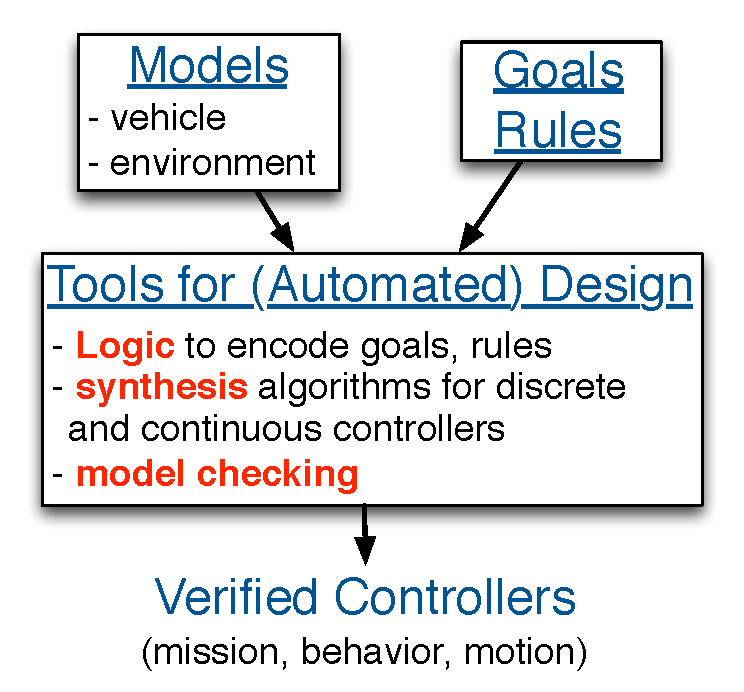
\includegraphics[width=2.5in]{correct-by-construction.pdf} 
   \caption{correct by construction example}
   \label{fig:correct-by-construction}
\end{figure}

These concepts have been extended to using probabilistic model checkers, and this work is most applicable to the concepts proposed in this think piece. Typically, an off-the-shelf model checking software such as PRISM~\cite{Kwiatkowska2001,prism} is used to find the probabilities of satisfying the desired set of logic based specifications. Given a full characterization of the system (known probabilities for environment and sensor models), model checking techniques can be used to find upper and lower bounds on the probability that the autonomy will satisfy the set of specifications.

Figure~\ref{fig:taxi-taxi} shows a recent example of a taxi driver with a specification on collision probability~\cite{johnson2012execution}. In this case, the authors have defined collision probability based on the current location density of an object (e.g.\ another car) in an environment, a map of the road structure, and a temporal/probabilistic prediction of the location density into the future, based on typical driving standards (Figure~\ref{fig:taxi-taxi}(left)). A collision bound is then calculated and used as a design specification for the controller. A controller can then be generated by selecting a `desired probability of collision', and generating and  checking a controller for the taxi driving in an environment with other cars. Figure~\ref{fig:taxi-taxi}(right) shows the case when the other cars in the environment are modeled as not obeying any rules of the road.By selecting a `desired probability of collision' and generating a controller, different autonomous driving behaviors can be realized, such as conservative driving or agressive driving. 


\begin{figure}[h] 
\centering
   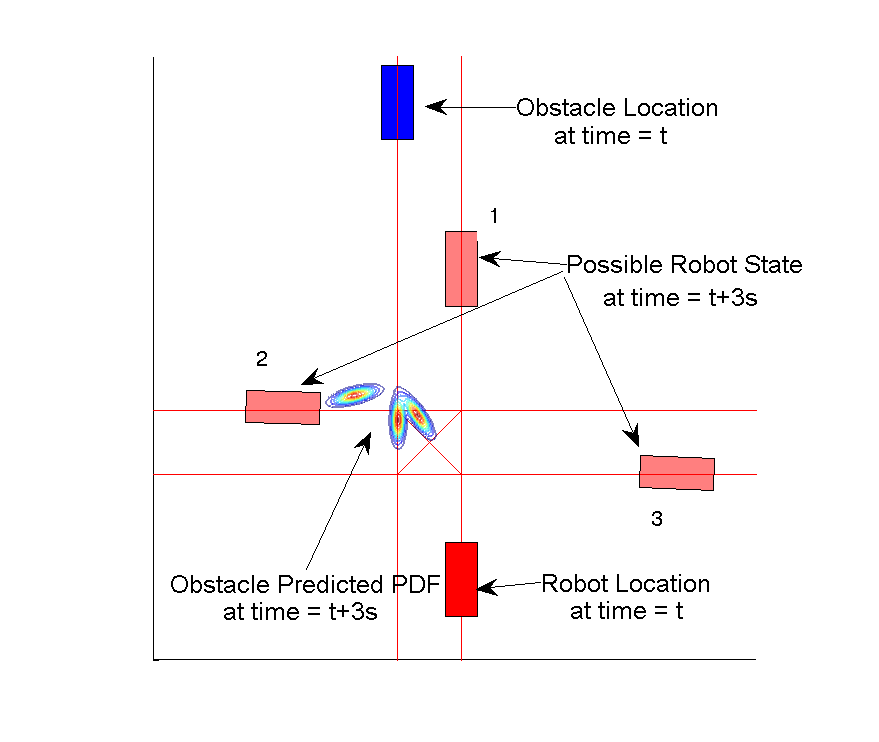
\includegraphics[width=3.0in]{coll_prob_inst.pdf} 
  % \label{fig:collision}
   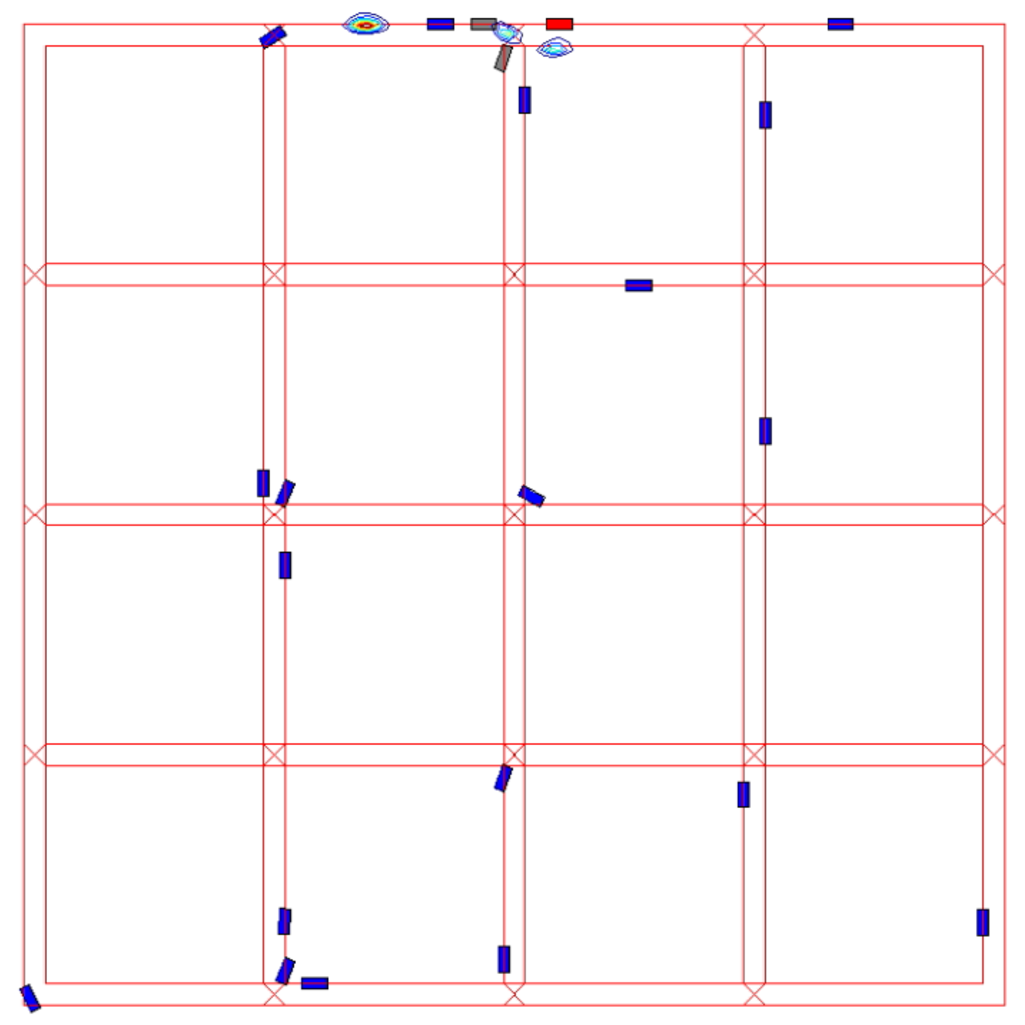
\includegraphics[width=2.5in]{taxi-driver.pdf} 
   \caption{collision probability taxi driver example}
   \label{fig:taxi-taxi}
\end{figure}

Given that there are now approaches to generating software for autonomous systems that are probabilistically correct, can we now begin to include human interaction (and models of humans) such that the controllers are designed with humans in mind?

\subsection*{Probabilistic modeling and humans}

Modeling even a portion of human capabilities will enable the ability to plan and optimize an integrated human-autonomy system. Modeling human-machine interactions in large-scale networked systems can be useful in making research more prospective, rather than reactive, which has typically been the characteristic of previous research on humans and automation. Modeling can also inform the design of future interfaces to support operators of multiple UV systems in the presence of concurrent operational and cognitive uncertainties. 

Research in modeling of human capabilities has been on-going to many years, from the early work on simple cognitive functions and interaction with autonomy~\cite{Sheridan92}, to more recent work attempting to model extensive cognitive capabilities~\cite{anderson1997act} and even the brain~\cite{brain2013}. Integrated databases have been developed for modeling/prediction of perception and motor skills~\cite{epic,Kieras99a,Byrne03a,actrpm}. Currently, these databases are focused on low level human skills, and do not integrate with the environment (such as the use of autonomy models). ACT-R~\cite{anderson1997act} is a cognitive architecture attempting to model a full range of human cognitive tasks, including the way we perceive, think about, and act on the world. The ACT-R architecture has developed modules  representing perceptual attention, motor programming, long-term declarative memory, goal processing, mental imagery and procedural competence. Applications have included air traffic control~\cite{lebiere2001multi,taatgen2006modeling} and multiple agents in military environments~\cite{best2006cognitive}. 


The human factors community, on the other hand, has focused on empirically driven tests in order to gain insightful observation of trends, but not formal models; one fruitful area has been in supervisory control of UAVs where several human operators are typically required to control current unmanned aerial vehicle (UAV) platforms~\cite{cooke2006human,cummings2007operator}.  Given the goal of one operator to many UAVs, automation support, even if imperfect, is mandated~\cite{barnes2010human,parasuraman2005flexible,parasuraman2009adaptive}. However, the extra task load generated by handling imperfect automation may interfere with adequately supervising a larger number of UAVs. Recent estimates of an operator's capacity to control multiple UAVs range from 1 to 16~\cite{Wickens2006},  
 but more precise estimates may be calculated by considering the impact of UAV coordination demands, UAV interaction and neglect times, automation reliability, mission type and operator tasks and the task-to-robot ratio~\cite{Wickens2006,cummings2008predicting,de2011adaptive,galster2006managing,parasuraman1997humans}. Research on operators in Air Traffic Control~\cite{Galster01a,Rantanen04a} has provided valuable insight into how users make decisions as a function of parameters such as stress, interface type, and time. 
These works typically derive key performance metrics from trends in the data, but do not formally model them. 

Many generic `non-cognitive' probabilistic models have been proposed as alternatives to well-known detailed cognitive computational models for predicting human-in-the-loop performance in networked unmanned vehicle applications. In \cite{Fan10} and \cite{Heger06}, for instance, human operators are modeled dynamically via probabilistic Markov models in order to capture random transitions between abstract discrete states that influence decision-making and task performance metrics. In \cite{Donmez10}, discrete-event task simulations with probability distributions on operator servicing times are used to explicitly model the performance effects of changing workload and vehicle utilization in a multi-UAV supervisory task. Both cognitive and non-cognitive dynamic probabilistic human-operator models can be used to generate sample-based performance prediction statistics via repeated random simulations of closed-loop task execution, and as such can provide useful insight into specific scenarios that lead to good/bad operator performance. However, such dynamic probabilistic models require a high level of detail and much training data to explicitly account for the effects of various task/network-related factors (e.g.\ number of agents, task load). These models also do not explicitly account for individual factors, e.g.\ differences in working memory capacity. Furthermore, many simulations must be run with dynamic models in order to make performance predictions for a single set of operating conditions, which can be cumbersome for exploring many different network/task conditions. 

A new class of probabilistic models has recently been developed that are potentially useful for prediction and verification of human operator performance in human-autonomysystems, either in the sense of performing detailed analyses related to dynamical process simulations or performing gross `high-level' analyses of human-machine system performance that abstract away certain dynamical details. Two of these models, \emph{Gaussian Process (GP) regression} and \emph{Bayesian networks (BN)}, can enable direct `function-like' performance  predictions without requiring simulations or an explicit model of the operator's decision-making processes \cite{Ergo}. Any expected variability arising from differences in these and other unmodeled factors related to task dynamics are described by the estimated probabilities associated with each prediction. A third type of model,  \emph{probabilistic discriminative classification models}, can be used to capture stochastic \emph{non-Markovian state-dependent switching behaviors} for discrete supervisory decision making by human operators in detailed process models \cite{Bourgault2007}, \cite{Ahmed2008}, \cite{Ahmed2011a}, which is currently not realizable with the probabilistic Markov or discrete event models mentioned above. 

As an example, consider the case of probabilistically modeling human observations at a macro level (human observations and/or tasks), in an effort to more formally exchange information with an autonomous system. Both discrete~\cite{Ahmed2012a} and continuous human inputs~\cite{Bourgault2008} have been modeled, including a rich set of structured inputs such as  `The target is near the tree and heading quickly toward you' or `There is nothing behind the wall.'  The key challenge is probabilistically modeling terms such as `near' or `behind'. 

Leveraging the fact that discrete random variables nicely represent soft (human) categorical information, the human information has been shown to be well-modeled via probabilistic classifiers  \cite{Ahmed-TRO-2012, Ahmed-ICRA-2010, Ahmed-ACC-2011a,Ahmed10SigPro}.  These classifiers are typically learned from human observation data, such as computer point and click; chat inputs; and natural language processing. Figure~\ref{fig:likelihood} shows a simple example of learning soft human categorical information from data.

\begin{figure}[h] 
\centering
   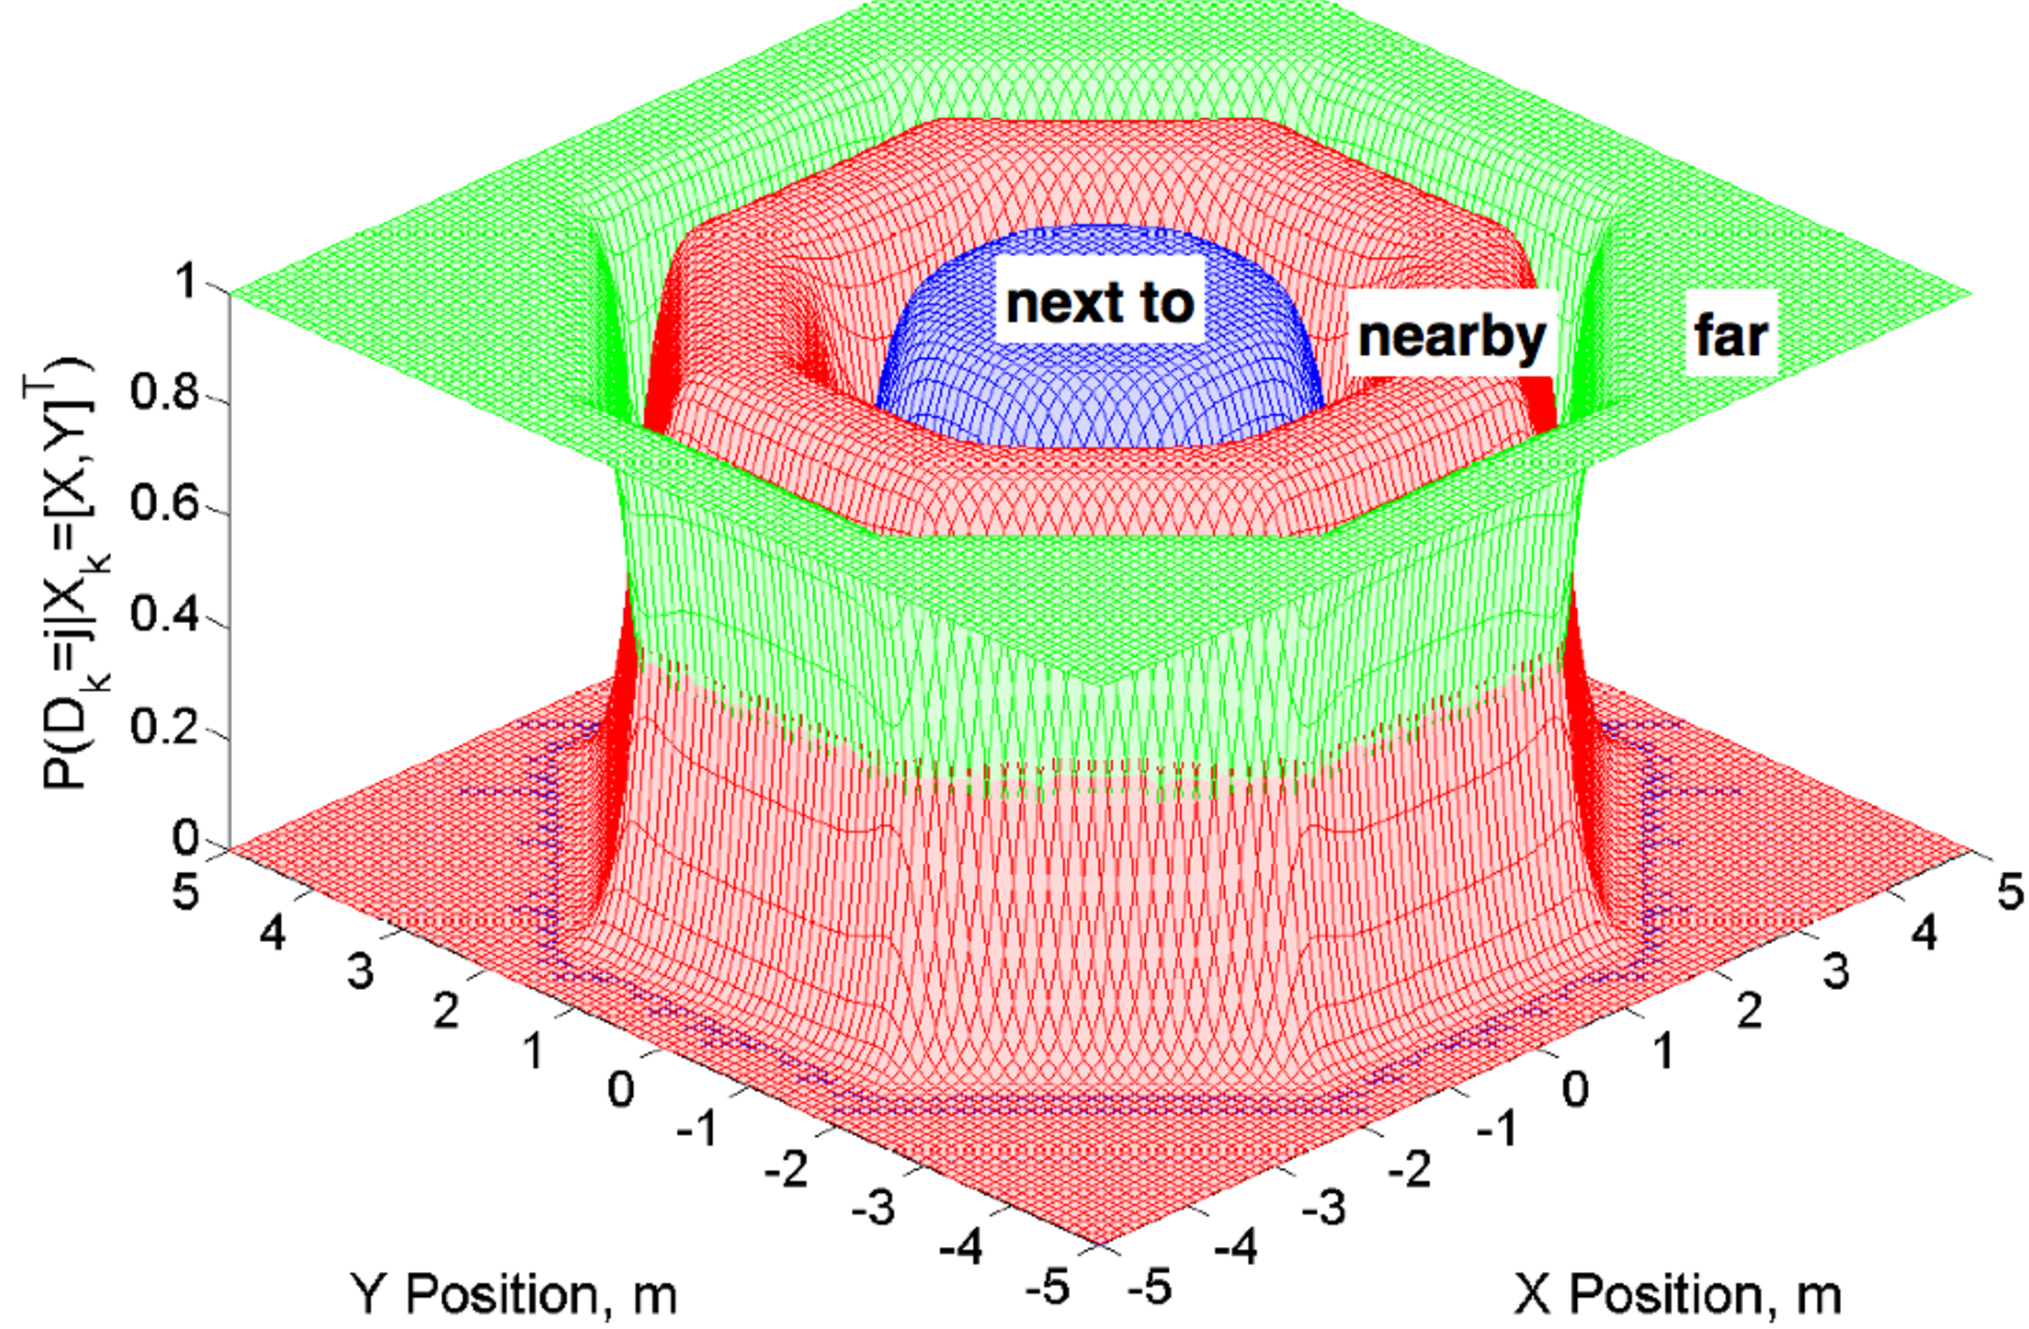
\includegraphics[width=3.5in]{mms.pdf} 
   \caption{Learned likelihood model for relations `next to', `nearby', and `far.' }
   \label{fig:likelihood}
\end{figure}

These likelihood functions then enable a host of subsequent functions, from cooperative planning to information fusion and inference. Ref.~\cite{Ahmed10SigPro} empirically investigates how human information can be used by an autonomous robot in a search mission. Even though  human subjects could not directly command robots, it was found that fusing human and robot observations greatly improved object search performance (i.e.\ number of targets found, time to find objects, object localization error) compared with baseline searches using robot observations alone. Human observations were particularly useful for correcting missed object detections and reducing the distances traveled by the robot, whereas the use of \textit{negative information} (e.g., `Nothing is near the bridge') was shown to be particularly important in the integrated human+robot team performance.

The use of Gaussian Process models has been shown to be particularly insightful into human tasking, including variations over users. In a collaboration between researchers in the human factors community and the autonomy community, collected operator data was modeled using different statistical modeling methods to study the ability to predict human operator performance in an  air defense simulation scenario~\cite{Ahmed2013a}; performance metrics were modeled as a function of task load, message quality, and operator working memory capacity. It was found that state-of-the-art Gaussian Process (GP) regression models can make predictions with uncertainty bounds that are more informative than traditional linear regression and discrete Bayesian network (BN) prediction models. More specifically, off-line tests of human operator metrics (such as working memory) are predictive in eventual performance of the operators in the UAV tasking environment (such as red zone performance). The GP models also nicely capture uncertainty in area of the model with little date, and trends/anomalies with user capabilities. Figure~\ref{fig:prob-humans} shows an example of one such predictive model, where task performance is captured as a function of working memory, which can be evaluated off-line in a priori tests. Several studies have shown that individual differences in working memory capacity play a major role in determining how well a person can focus attention on visual tasks and cope with distractors such as irrelevant messages~\cite{Engle02}. More generally, working memory is thought to be a key component of executive control processes that underlie effective multi-tasking and decision-making in time-critical tasks~\cite{Parasuraman2010,Endsley95}. Therefore, individual differences in working memory capacity could be modeled and used in developing verifiable specifications. 

\begin{figure}[h] 
   \centering
   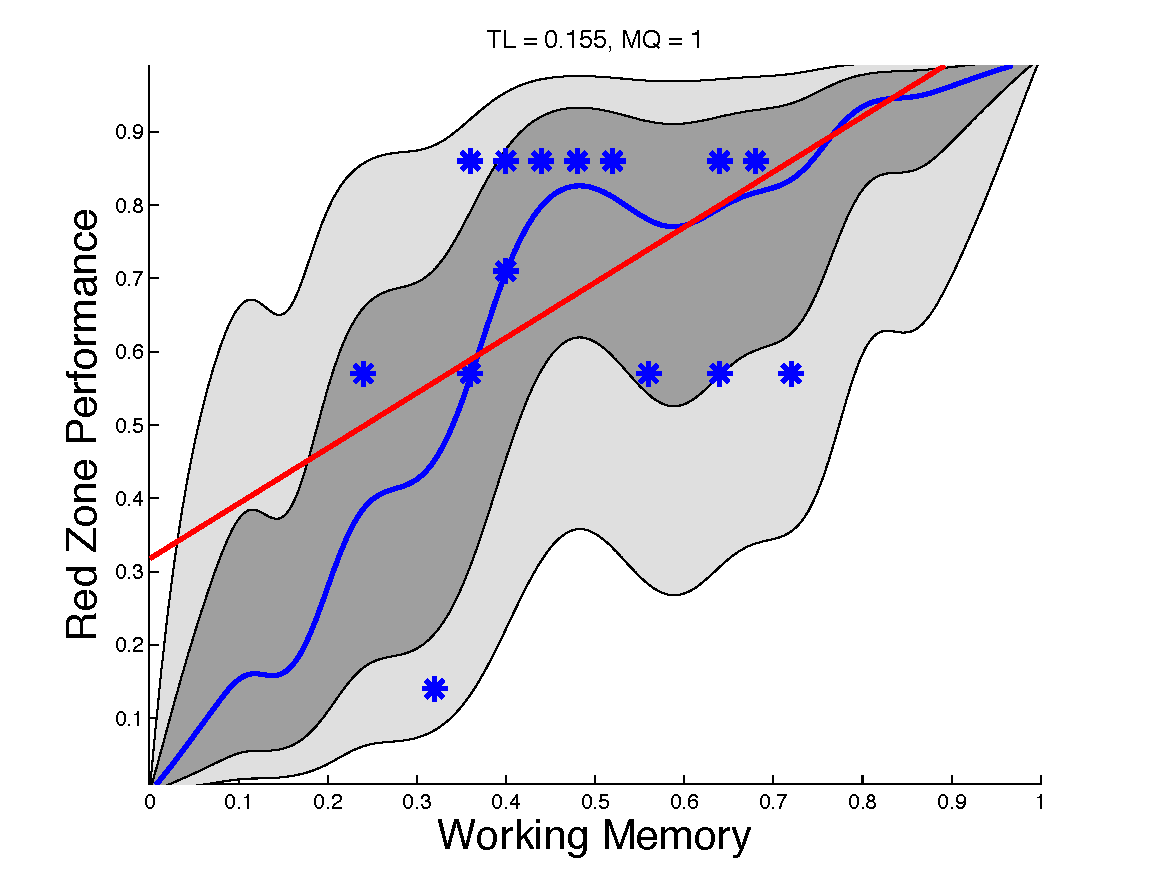
\includegraphics[width=3.5in]{GP-fig.pdf} 
   \caption{Example of probabilistic modeling of human capabilities, correlating performance with working memory.}
   \label{fig:prob-humans}
\end{figure}

In summary, there are many classes of models of human tasking, behaviors, and decision making. Importantly, there is a growing maturity in probabilistic models of human decision making can could enable fundamental studies in formal verification of human-autonomy systems. 


\subsection*{Collaborative autonomy}

\mc{TODO write this section.  Then revised by Ella.}

Collaboration over computation, communication, navigation, and sensing

Multi-vehicle collaboration 
Decentralized task selection / allocation (Market protocols - Wellman et al, Optimization - How et al) 
Cooperative path planning (Tsourdos et al)
Scalability through swarm-based techniques (e.g., consensus, potential field)  (McLain et al)

Collaborative human-autonomy systems
Human intent prediction (e.g. partially-observable Markov Decision Process) (Karami et al)
Adaptive tasking (Parasuram et al)
Use metrics (e.g., confidence) to decide when to ask for help (Fong et al) 
Apply perspective-taking to project companion awareness state (Trafton et al)


Capable strategies for collaborative autonomy systems exist and can be 
leveraged for co-design of human-autonomy systems


\subsection*{Model-based system engineering}

\ella{TODO}

Transition from functional decomposition..
Does not scale well
Difficult to verify


…to Model-based System Engineering 
State-based models of each actor are generated.
Each model is re-used over all phases of system engineering
Improves scalability and consistency
State analysis offers a formal method to verify behaviors
Successfully applied to single-actor systems (e.g., spacecraft missions)

